\section{Empirical Error and Overfitting}

\section{Assessment}

\section{Performance Measurement}
\subsection{Error Rate and Accuracy}
Error rate is the most direct measurement of performance. It is defined as the ratio of misclassified examples,
i.e.
$$err(f; D) = \frac{1}{m} \sum_{i=1}^m \mathbb{I}(f(\V{x}_i) \neq y_i)$$
where $m$ is the total number of examples. The accuracy is just the complement of error rate:
$$acc(f; D) = 1 - err(f; D)$$
Generally, for a distribution $\mathcal{D}$ over a data set $D$ with pdf (pmf) $p$, the error rate is defined as
\begin{equation}
    err(f;\mathcal{D}) = \int_{\V{x} \sim \mathcal{D}}\mathbb{I}(f(\V{x}) \neq y) p(\V{x})\diff{\V{x}}
\end{equation}

\subsection{Precision, Recall and F1 Score}
% Confusion matrix of classification.
\begin{table}[ht]
\begin{center}
    \begin{tabular}{|c|c|c|}\hline
        \diagbox{Fact}{Prediction} & Positive & Negative\\
        \hline
        True & TP & FN\\
        \hline
        False & FP & TN\\
        \hline
    \end{tabular}
\end{center}
\caption{Confusion Matrix}
\end{table}

Let $T$ and $F$ be the number of \textbf{true} and \textbf{false} examples respectively. Let $P$ and $N$ be
the number of \textbf{positive} and \textbf{negative} examples respectively. Then we have $m = P + N = T + F$
where $m$ is the number of total examples, and\marginnote{Look at the columns of the\\ confusion matrix.}
\begin{equation}
    \begin{cases}
        P &= TP + FP\\
        N &= FN + TN
    \end{cases}
\end{equation}
and\marginnote{Look at the rows of the\\ confusion matrix.}
\begin{equation}
    \begin{cases}
        T &= TP + FN\\
        F &= FP + TN
    \end{cases}
\end{equation}
The \textbf{precision} is defined as\marginnote{Of those positive examples, how many are truly positive? }
\begin{equation}
    p = \frac{TP}{P} = \frac{TP}{TP + FP}
\end{equation}
The \textbf{recall} is defined as\marginnote{How many truly positive \\examples have been picked out?}
\begin{equation}
    r = \frac{TP}{T} = \frac{TP}{TP + FN}
\end{equation}

% precision-recall curve.
\begin{figure}[ht]
    \begin{center}
    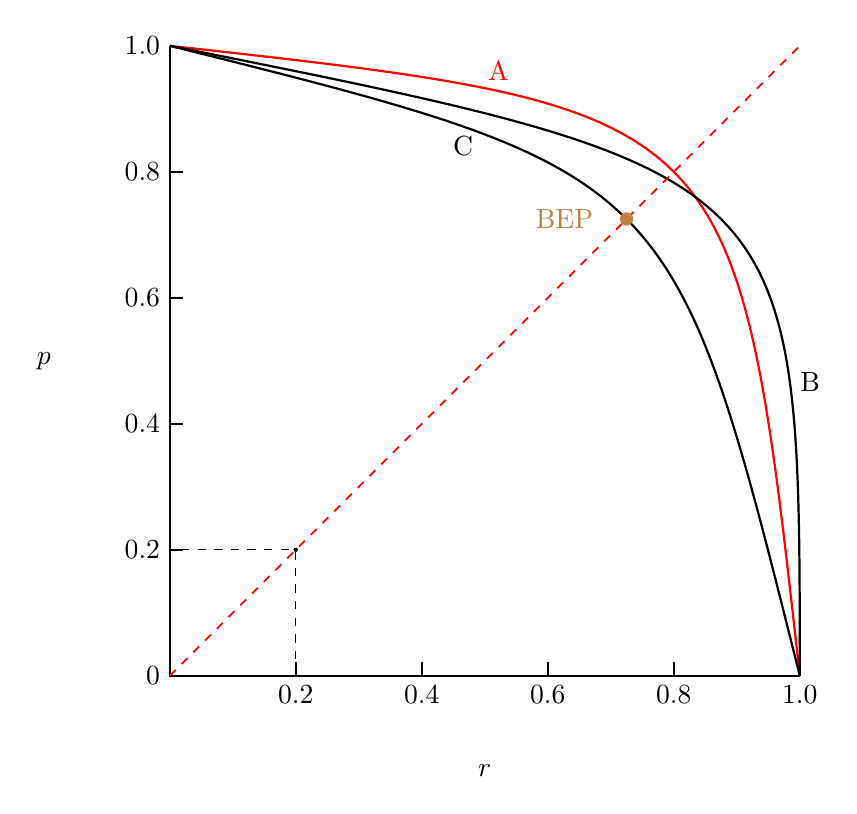
\begin{tikzpicture}[scale=8]
        \draw [thick] (0, 1) -- (0, 0) -- (1, 0);
        % \draw [thick] (0, 1) to [out=-30, in=110] (1, 0);
        % \draw [thick] (0, 1) to [out=-10, in=90] (1, 0);
        % \draw [thick, red] (0, 1) to [out=0, in=105] (1, 0);
        \draw [red, thick] (0, 1) .. controls (0.9, 0.9) .. (1, 0) node[above, near start] {A};
        \draw [thick] (0, 1) .. controls (1.0, 0.8) .. (1, 0) node[right, near end] {B};
        \draw [thick] (0, 1) .. controls (0.8, 0.8) .. (1, 0) node[below, near start] {C};
        \draw [semithick, red, domain=0:1, dashed] plot (\x, \x);
        \draw[dashed] (0.2, 0) -- (0.2, 0.2) -- (0, 0.2);

        \foreach \x in {0.2, 0.4, 0.6, 0.8} {
            \draw (\x, 0) node[below] {$\x$} [thick] -- ++(0, 0.6pt);
            \draw (0, \x) node[left] {$\x$} [thick] -- ++(0.6pt, 0);
        }
        \node [left] at (0, 0) {$0$};
        \node [below] at (1, 0) {$1.0$};
        \node [left] at (0, 1) {$1.0$};
        \node at (0.5, -0.15) {$r$};
        \node at (-0.2, 0.5) {$p$};
        % \draw [fill=magenta] (0.725, 0.725) circle [radius=0.01];
        % \node [left] at (0.725, 0.725) {BEP};
        \fill [brown] (0.725, 0.725) circle (0.3pt) node[left=0.3cm] {BEP};
        \fill (0.2, 0.2) circle (0.1pt);
    \end{tikzpicture}
    \end{center}
    \caption{Precision-Recall Curve}\label{pr_curve}
\end{figure}
In many algorithms, for example the logistic regression, we first compute a value from the given feature
vector of an example, then we compare it
with a threshold value to determine whether it is positive or negative. In order to get high recall, we can
mark all examples as positive (that is, set the threshold value to a very small value), which makes $FN = 0$;
but this will make the precision low since all false examples are classified as positive too.
Similarly, in order to achieve high precision, we can set the threshold value large (that is, we only classify
an example as positive if we are confident enough), but this will leave many examples as negative, hence $FN$
is large, which causes low recall. In general, precision and recall can not both increase at the same time.
See figure~\ref{pr_curve}.\marginnote{For example, B performs better than C in figure~\ref{pr_curve}.} If one
learner's P-R curve is enclosed  by anothers', then the latter has a better performance. In other situations,
can use the \textbf{B}reak \textbf{E}vent \textbf{P}oint to compare two learners' performance. Here, the BEP
is just the point where precision equals recall. See figure~\ref{pr_curve} for an example.

The F1 score is defined as
\begin{equation}
    F1 = \frac{2}{\frac{1}{p} + \frac{1}{r}} = \frac{2pr}{p + r}
\end{equation}


\subsection{ROC and AUC}

\textbf{True/False Positive Rate} is defined as
\begin{equation}
    \begin{cases}
        TPR &= \dfrac{TP}{T} = \dfrac{TP}{TP + FN}\vspace{5pt}\\
        FPR &= \dfrac{FP}{F} = \dfrac{FP}{FP + TN}
    \end{cases}
\end{equation}
The \textbf{R}eceiver \textbf{O}perating \textbf{C}haracteristic curve uses true positive rate as vertical
axis and false positive rate as horizontal axis. Below is a ROC curve and the gray area is the
corresponding \textbf{A}era \textbf{U}nder \textbf{C}urve.
% ROC curve and AUC.
\begin{figure}[ht]
    \begin{center}
    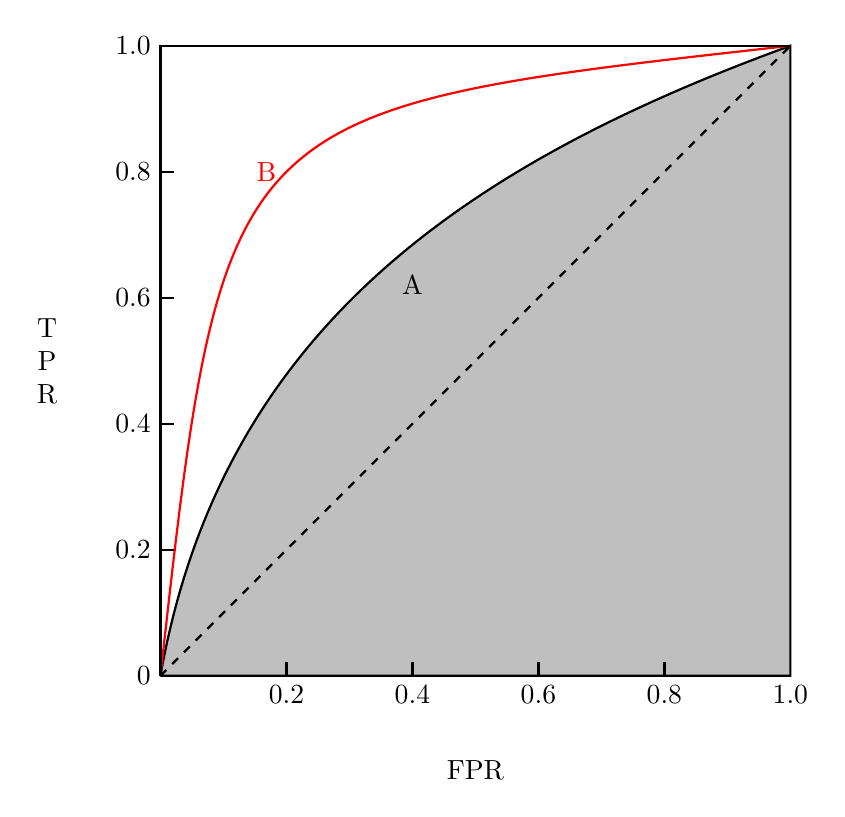
\begin{tikzpicture}[scale=8]
        \draw[thick, fill=lightgray] (0, 0) to [out=80, in=200] (1, 1) -- (1, 0) -- (0, 0);
        \draw[thick, red] (0, 0) .. controls (0.1, 0.9) .. (1, 1) node[left, midway]{B};
        \draw[dashed, thick] (0, 0) -- (1, 1);
        \draw[thick] (0, 0) -- (0, 1) -- (1, 1);

        \foreach \x in {0.2, 0.4, 0.6, 0.8} {
            \draw (\x, 0) node[below] {$\x$} [thick] -- ++(0, 0.6pt);
            \draw (0, \x) node[left] {$\x$} [thick] -- ++(0.6pt, 0);
        }
        \node [left] at (0, 0) {$0$};
        \node [below] at (1, 0) {$1.0$};
        \node [left] at (0, 1) {$1.0$};
        \node [below] at (0.4, 0.65) {A};
        \node at (0.5, -0.15) {FPR};
        \node [align=center] at (-0.18, 0.5) {T\\P\\R};
        \end{tikzpicture}
    \end{center}
    \caption{ROC Curve}\label{ROC}
\end{figure}

When $TPR = FPR$, we have
$$\frac{TP}{T} = \frac{FP}{F}$$
Notice that $T = TP + FN$ and $F = FP + TN$, we have
$$\frac{FN}{T} = \frac{TN}{F}$$
That is, for any example, we predict it to be positive with a given probability. So in figure~\ref{ROC}, the
dashed diagonal corresponds to the random guess model (with a fixed probability). When $(FPR, TPR) = (1, 0)$,
we have
\begin{equation*}
    \begin{cases}
        TP &= 0\\
        TN &= 0
    \end{cases}
\end{equation*}
that is, $acc = 0$. When $(FPR, TPR) = (0, 1)$, we have
\begin{equation*}
    \begin{cases}
        FP &= 0\\
        FN &= 0
    \end{cases}
\end{equation*}
that is, $acc = 1$. When $(FPR, TPR) = (0, 0)$, we have
\begin{equation*}
    \begin{cases}
        FP &= 0\\
        TP &= 0
    \end{cases}
\end{equation*}
that is, the predictor marks all examples as negative. When $(FPR, TPR) = (1, 1)$, we have
\begin{equation*}
    \begin{cases}
        FN &= 0\\
        TN &= 0
    \end{cases}
\end{equation*}
that is, the predictor marks all example as positive.

Of course, if a learner's ROC is fully enclosed by anothers', then the latter has a better performance.
For example, in figure~\ref{ROC}, the learner with ROC B performs better than the one with ROC A.
If two learners' ROCs cross with each other, then we may compare their AUCs and again we prefer the one with
larger AUC\@.

\section{Bias and Variance}

Let's consider the bias and variance decomposition of supervised learning. Asssume $\mathcal{X}$ is the
instance space and $\mathcal{Y}$ the label space. Let $\p$ be the joint distribution over
$\mathcal{X} \times \mathcal{Y}$ and $p$ the joint pdf. Let \dataset\ be any i.i.d.\ dataset w.r.t.\ the
distribution $\p$, that is $D \sim \p^m$. For any given instance \V{x}, we have

\begin{df}[Expected label]
    The expected label of \V{x} is defined as:
    \begin{equation}
        \bar{y}(\V{x}) := \E_{y|\V{x}}[y] := \int_y y\,p(y|\V{x})dy
    \end{equation}
\end{df}

Notice that $\bar{y}(\V{x})$ is deterministic w.r.t.\ \V{x}, it is the true model that we want to approximate.
Naturally, the data-intrinsic noise is defined as:
\begin{equation}
    \E_{\V{x}, y}\left[{(\bar{y}(\V{x}) - y)}^2\right] = \int_{\V{x}} \int_y {(\bar{y}(x) - y)}^2 p(\V{x}, y)
    d\V{x}dy
\end{equation}
If we write the true model as $f(\V{x})$, then $y$ can be written as $y = f(\V{x}) + \varepsilon$ where
$\varepsilon$ is a random variable (for fixed \V{x}) \wrt $y$ \st $\E_{y}[\varepsilon] = 0$. If we assume that
$\varepsilon$ is independent of \V{x} and has variance $\sigma^2$, it is obvious from the above equation that
the data-intrinsic noise is just $\sigma^2$.

For any given algorithm $\mathcal{A}$, we can use it to train a learner $h_D = \mathcal{A}(D)$ from the
dataset $D$. Since $D$ is a random variable and $h_D$ is a function of $D$, $h_D$ is also a random variable.

\begin{df}[Expected learner]
    The expected learner given by the algorithm $\mathcal{A}$ on $m$ training examples is defined as:
    \begin{equation}
        \bar{h} := \E_{D \sim \p^m}[h_D] := \int_D h_D\, p(D) dD
    \end{equation}
\end{df}

\begin{df}[Variance]
    The variance of the learners given by the algorithm $\mathcal{A}$ on $m$ training examples is defined as:
    \begin{equation}
        \E_{\V{x}, D}\left[{(h_D(\V{x}) - \bar{h}(\V{x}))}^2\right]
    \end{equation}
\end{df}

\begin{df}[Bias]
    The bias of the algorithm $\mathcal{A}$ on $m$ training examples  is defined as the expected square error
    of the expected learner and the true model, i.e.
    \begin{equation}
        \E_{\V{x}}\left[{(\bar{h}(\V{x}) - \bar{y}(\V{x}))}^2\right]
    \end{equation}
\end{df}

For any given $h_D$, as usual we have

\begin{df}[Expected true error]
    The expected true error of a learner $h_D$ is defined as:
    \begin{equation}
        \E_{(\V{x}, y) \sim \p}\left[{(h_D(\V{x}) - y)}^2\right] = \int_{\V{x}} \int_y {(h_D(\V{x}) - y)}^2
        p(\V{x}, y) d\V{x} dy
    \end{equation}
\end{df}

Similar to the above expected true error \wrt to a specific learner, we can defined the expected true error
\wrt to an algorithm $\mathcal{A}$.

\begin{df}[Expected true error]
    The expected true error of an algorithm $\mathcal{A}$ is defined as:
    \begin{equation}
        \E_{\substack{(\V{x}, y) \sim \p \\ D \sim \p^m}}\left[{(h_D(\V{x}) - y)}^2\right] =
        \int_D \int_{\V{x}} \int_y {(h_D(\V{x}) - y)}^2 p(\V{x}, y) p(D) d\V{x} dy dD
    \end{equation}
\end{df}

In order to understand the expected true error of an algorithm, we can decompose it into three parts as
following:
\begin{align*}
    \E_{\V{x}, y, D}\left[{(h_D(\V{x}) - y)}^2\right] &= \E_{\V{x}, y, D} \left[{(h_D(\V{x}) - \bar{h}(\V{x})
    + \bar{h}(\V{x}) - y)}^2 \right] \\
    &= \E_{\V{x}, D} \left[{(h_D(\V{x}) - \bar{h}(\V{x}))}^2\right] +
    \E_{\V{x}, y}\left[{(\bar{h}(\V{x}) - y)}^2\right]\\
    &\quad\quad + 2\E_{\V{x}, y, D}\left[{(h_D(\V{x}) - \bar{h}(\V{x}))(\bar{h}(\V{x}) - y)}\right]\\
\end{align*}
Since
\begin{align*}
    \E_{\V{x}, y, D}\left[(h_D(\V{x}) - \bar{h}(\V{x}))(\bar{h}(\V{x}) - y)\right] &=
    \E_{\V{x}, y}\left[\E_D\left[(h_D(\V{x}) - \bar{h}(\V{x}))(\bar{h}(\V{x}) - y)\right]\right] \\
    &= \E_{\V{x}, y}\left[(\bar{h}(\V{x}) - y) \E_D\left[(h_D(\V{x}) - \bar{h}(\V{x}))\right]\right] \\
    &= 0
\end{align*}
we have:
\begin{equation}\label{bias-variance:1}
    \E_{\V{x}, y, D}\left[{(h_D(\V{x}) - y)}^2\right] = \E_{\V{x}, D} \left[{(h_D(\V{x}) -
    \bar{h}(\V{x}))}^2\right] + \E_{\V{x}, y}\left[{(\bar{h}(\V{x}) - y)}^2\right]
\end{equation}
Similarly,
\begin{align*}
    \E_{\V{x}, y}\left[{(\bar{h}(\V{x}) - y)}^2\right] &= \E_{\V{x}, y}\left[{(\bar{h}(\V{x}) - \bar{y}(\V{x})
    + \bar{y}(\V{x}) - y)}^2\right]\\
    &= \E_{\V{x}}\left[{(\bar{h}(\V{x}) - \bar{y}(\V{x}))}^2\right] +
    \E_{\V{x}, y}\left[{(\bar{y}(\V{x}) - y)}^2\right] \\
    &\quad\quad + 2\E_{\V{x}, y}\left[(\bar{h}(\V{x}) - \bar{y}(\V{x}))(\bar{y}(\V{x}) - y)\right]
\end{align*}
and
\begin{align*}
    \E_{\V{x}, y}\left[(\bar{h}(\V{x}) - \bar{y}(\V{x}))(\bar{y}(\V{x}) - y)\right] &=
    \E_{\V{x}}\left[\E_{y|\V{x}}\left[(\bar{h}(\V{x}) - \bar{y}(\V{x}))(\bar{y}(\V{x}) - y)\right]\right]\\
    &= \E_{\V{x}}\left[(\bar{h}(\V{x}) - \bar{y}(\V{x})) \E_{y|\V{x}}\left[(\bar{y}(\V{x}) - y)\right]\right]\\
    &= 0
\end{align*}
implies
\begin{equation}\label{bias-variance:2}
    \E_{\V{x}, y}\left[{(\bar{h}(\V{x}) - y)}^2\right] =
    \E_{\V{x}}\left[{(\bar{h}(\V{x}) - \bar{y}(\V{x}))}^2\right]
    + \E_{\V{x}, y}\left[{(\bar{y}(\V{x}) - y)}^2\right]
\end{equation}
Combine equation~\eqref{bias-variance:1} and~\eqref{bias-variance:2}, we have:
\begin{equation}\begin{split}
    \E_{\V{x}, y, D}\left[{(h_D(\V{x}) - y)}^2\right] &= \E_{\V{x}, D} \left[{(h_D(\V{x}) -
    \bar{h}(\V{x}))}^2\right] + \E_{\V{x}}\left[{(\bar{h}(\V{x}) - \bar{y}(\V{x}))}^2\right]\\
    &\quad\quad+ \E_{\V{x}, y}\left[{(\bar{y}(\V{x}) - y)}^2\right]
\end{split}\end{equation}
That is, the expected true error of an algorithm can be decomposed as the sum of the variance, the bias, and
the noise.